% Final presentation (deliverable vi). Compile with pdflatex from Doc/presentation/
% (figures are read from ../report/figures, produced by `run_evaluation.py report`).
\documentclass[aspectratio=169,11pt]{beamer}
\usetheme{default}
\usecolortheme{dove}
\setbeamertemplate{navigation symbols}{}
\setbeamertemplate{footline}[frame number]
\usepackage{amsmath,amssymb,booktabs}
\graphicspath{{../report/figures/}}
\newcommand{\Reg}{\mathrm{Reg}}

\title{Learning to Bid Under a Budget}
\subtitle{A Batched First-Price Ad Auction with Unknown Click Probabilities}
\author{Vivek Raj \and Anvit Aggarwal \and Eshaan Ashish Jaiswal \and Gella Naga Sai Krishna}
\institute{IIT Gandhinagar --- CS329 Foundations of AI, Group 22}
\date{}

\begin{document}

\begin{frame}
  \titlepage
\end{frame}

% ---------------------------------------------------------------------------
\begin{frame}{The question}
  \begin{itemize}
    \item $m$ advertisers, $n$ users, $T$ rounds. Each round every advertiser submits a \emph{full bid
          vector} with $\sum_j b_{ij}\le B_i$; highest bid on each user wins and pays its bid
          (first price).
    \item A click on $u_j$ is worth $v$ and happens with probability $f_{ij}$, which is
          \textbf{unknown} and must be learned from won impressions only (semi-bandit feedback).
  \end{itemize}
  \vspace{1em}
  \begin{block}{Guiding question}
    How much do advertiser profit and allocation efficiency suffer when $f$ must be learned online,
    and how does the gap change when \emph{all} advertisers learn at once?
  \end{block}
\end{frame}

\begin{frame}{Known $f$: best response is a 0--1 knapsack}
  Against competing bids $c_{-i,j}=\max_{k\ne i}b_{kj}$, winning $u_j$ costs $c_{-i,j}+1$:
  \[
    \max_{x\in\{0,1\}^n}\sum_j\big(f_{ij}v-c_{-i,j}-1\big)x_j
    \quad\text{s.t.}\quad\sum_j(c_{-i,j}+1)x_j\le B_i ,
  \]
  solved exactly by dynamic programming in $O(nB_i)$.
  \vspace{0.8em}
  \begin{itemize}
    \item Learners (Algorithm 1) replace $f_{ij}$ with an index $\tilde f_j$:
          UCB $\min\{1,\hat f_j+\sqrt{\alpha\ln t/N_j}\}$ or a Thompson sample from
          $\mathrm{Beta}(1+s_j,1+N_j-s_j)$.
    \item With $v=1$ and integer bids every item value is $\le 0$, so nobody bids; we use $v=5$.
  \end{itemize}
\end{frame}

\begin{frame}{Three tiers, one assumption relaxed at a time}
  \begin{description}[Tier 3]
    \item[Tier 1] $f$ known. Reference equilibrium $b^*$ (best-response dynamics, fictitious play,
          support enumeration) and the omniscient planner. \hfill\emph{Vivek}
    \item[Tier 2] One learner vs.\ opponents fixed at $b^*_{-i}$: a budgeted combinatorial
          semi-bandit. UCB, Thompson, greedy, $\epsilon$-greedy, budget-paced. \hfill\emph{Anvit}
    \item[Tier 3] All advertisers learn concurrently; non-stationary market. \hfill\emph{Eshaan}
  \end{description}
  \vspace{0.6em}
  Shared evaluation harness and sensitivity study \hfill\emph{Sai Krishna}
  \begin{itemize}
    \item Any agent implementing \texttt{BaseAdvertiserAgent} runs unchanged in every tier.
    \item Grid $m\in\{2,3,5\}$, $n\in\{5,10,20,50\}$, $\kappa\in\{0.1,0.25,0.5,1\}$;
          canonical / discounted / cumulative budgets; 30 seeds, 95\% CIs; $T=10^3$ (and $10^4$).
  \end{itemize}
\end{frame}

\begin{frame}{Metrics (all computed with the true $f$)}
  \begin{itemize}
    \item Regret $\Reg_T=\sum_t\big(p_i^*(c^t_{-i})-p_i(b^t)\big)$ and its log--log slope
          ($<1$ means sublinear).
    \item Equilibrium gap $\varepsilon_t=\max_i\big(p_i^*(c^t_{-i})-p_i(b^t)\big)$ and
          $\|b^t-b^*\|_1$.
    \item Efficiency $\mathrm{Eff}_t$: share of users won by their highest-$f$ advertiser.
    \item Revenue, welfare, advertiser profit; price of learning = Tier 1 $-$ learned.
    \item Cumulative budgets: regret against the fluid LP (bandits-with-knapsacks) benchmark.
  \end{itemize}
\end{frame}

% ---------------------------------------------------------------------------
\begin{frame}{Tier 1: scarce budgets cost efficiency even at equilibrium}
  \begin{columns}[T]
    \begin{column}{0.6\textwidth}
      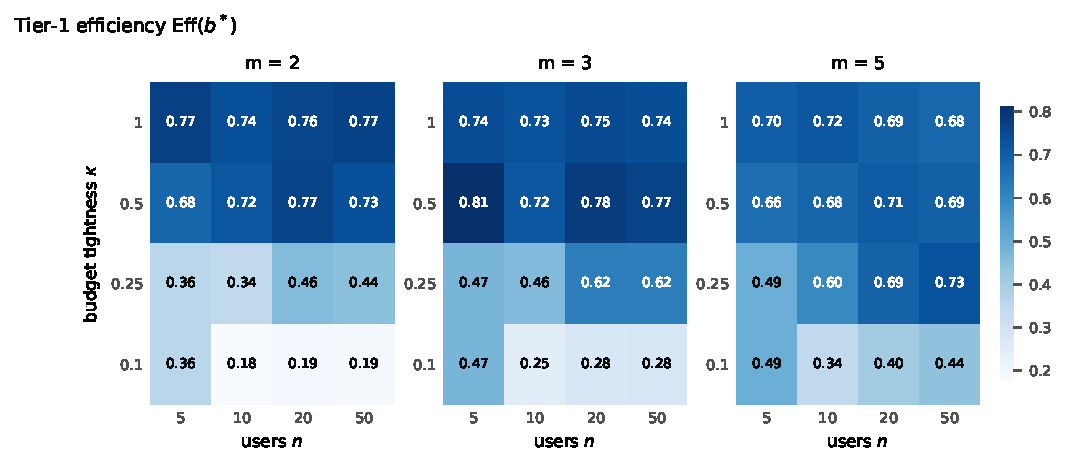
\includegraphics[width=\linewidth]{tier1_t1_efficiency.pdf}
    \end{column}
    \begin{column}{0.38\textwidth}
      \small
      \begin{itemize}
        \item $\kappa=0.1$: only 18--49\% of users go to their best advertiser; 66--81\% at
              $\kappa\ge0.5$.
        \item Pure equilibria certified in 80\% of instances, but only 0--33\% for $m=5$,
              $n\ge20$.
        \item Even with known $f$, simultaneous best response \emph{cycles}: final gap
              $0.76/1.42/2.37$ for $m=2/3/5$.
      \end{itemize}
    \end{column}
  \end{columns}
\end{frame}

\begin{frame}{Tier 2 (H1): regret is sublinear; Thompson learns fastest}
  \begin{columns}[T]
    \begin{column}{0.6\textwidth}
      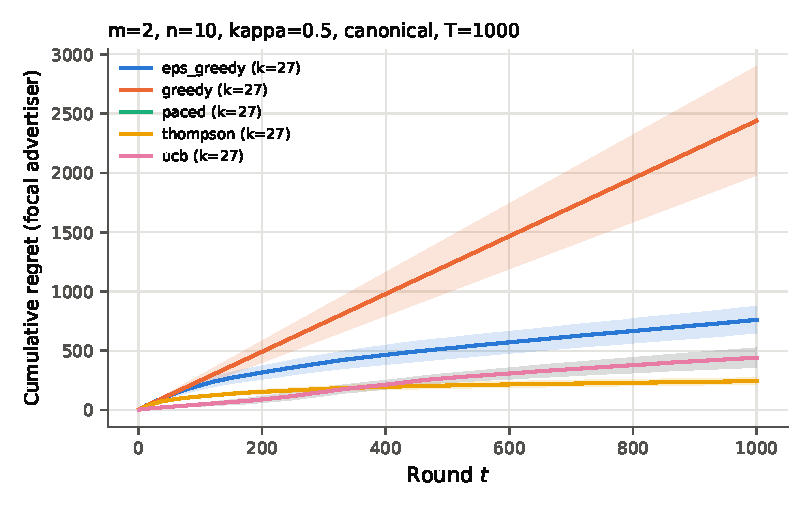
\includegraphics[width=\linewidth]{tier2_curves_cum_regret.pdf}
    \end{column}
    \begin{column}{0.38\textwidth}
      \small
      \begin{itemize}
        \item Thompson has the lowest regret in \textbf{all 47} cells with a pure equilibrium.
        \item Regret per round: 0.49 (TS), 1.22 ($\epsilon$-gr.), 1.77 (UCB), 2.95 (greedy).
        \item Log--log slopes 0.33 / 0.66 / 0.73 / 0.79; greedy tends to linear for $n\ge 20$.
      \end{itemize}
    \end{column}
  \end{columns}
\end{frame}

\begin{frame}{H1 at $T=10^4$, and how much UCB's $\alpha$ matters}
  \begin{columns}[T]
    \begin{column}{0.55\textwidth}
      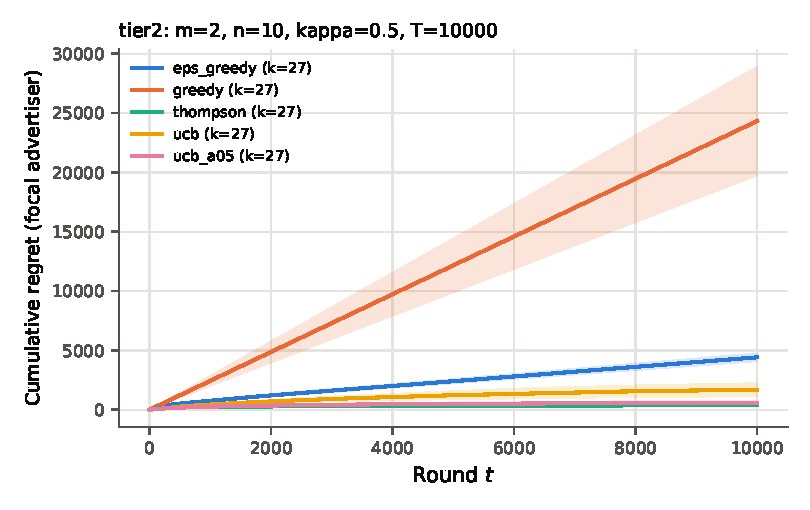
\includegraphics[width=\linewidth]{tier2_long_cum_regret_m2_n10.pdf}
    \end{column}
    \begin{column}{0.43\textwidth}
      \small
      Regret log--log slope at $T=10^4$ ($m\in\{2,3\}$, $n\in\{10,20\}$):\\[0.3em]
      \begin{tabular}{@{}lc@{}}
        \toprule
        Thompson & 0.17--0.22 \\
        UCB, $\alpha=0.5$ & 0.23--0.38 \\
        UCB, $\alpha=2$ & 0.50--0.58 \\
        $\epsilon$-greedy & $\approx 0.8$ \\
        greedy & 1.00 (linear) \\
        \bottomrule
      \end{tabular}\\[0.5em]
      At $T=10^3$, lowering $\alpha$ from 2 to 0.5 cuts UCB's regret by 59\%; Thompson is still
      best in 43 of 47 cells.
    \end{column}
  \end{columns}
\end{frame}

\begin{frame}{H3: tight budgets do \emph{not} slow learning}
  \begin{itemize}
    \item Thompson's regret per round is flat in $\kappa$ (0.45--0.53).
    \item UCB's regret \emph{grows} with $\kappa$ (0.81 at $\kappa=0.25$ to 3.38 at $\kappa=1$):
          a bigger budget buys more optimistic, exploratory impressions.
    \item The efficiency loss at tight budgets is already present in Tier 1, so H3 must be read
          relative to $b^*$, not in absolute terms.
  \end{itemize}
\end{frame}

\begin{frame}{Tier 3 (H2): the gap grows with $m$; Thompson damps cycling}
  \begin{columns}[T]
    \begin{column}{0.6\textwidth}
      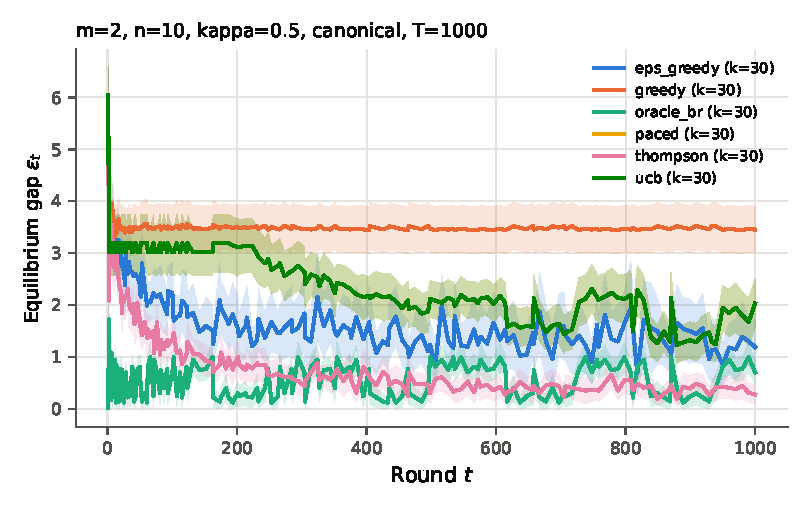
\includegraphics[width=\linewidth]{tier3_curves_eq_gap.pdf}
    \end{column}
    \begin{column}{0.38\textwidth}
      \small
      \begin{itemize}
        \item Final $\varepsilon$ for $m=2/3/5$: Thompson $0.67/1.25/2.48$; UCB $2.3/3.7/4.9$;
              known-$f$ best response $0.76/1.42/2.37$.
        \item H2 supported: the gap widens with the number of advertisers.
        \item At $T=10^4$ the gap keeps shrinking for UCB and Thompson; greedy stays locked in.
        \item Price of learning (Thompson): $-0.02$ efficiency, $-2.6$ revenue per round;
              advertisers' profit slightly \emph{rises}.
      \end{itemize}
    \end{column}
  \end{columns}
\end{frame}

\begin{frame}{Robustness across round structures}
  \small
  \begin{tabular}{@{}lccc@{}}
    \toprule
    & canonical & discounted ($\gamma=0.999$) & cumulative ($\rho=0.5$) \\
    \midrule
    Tier-2 best learner (cells won) & Thompson (47/47) & Thompson (47/47) & Thompson 26, paced 13 \\
    Thompson regret slope & 0.33 & 0.25 & 19.5 \\
    Paced regret slope & 0.73 & 0.59 & \textbf{2.7} \\
    Tier-3 gap, Thompson ($m=2/3/5$) & 0.67/1.25/2.48 & same & 4.98/4.76/4.09 \\
    Tier-3 gap, paced ($m=2/3/5$) & 2.32/3.67/4.93 & same & \textbf{2.52/3.21/3.89} \\
    \bottomrule
  \end{tabular}
  \vspace{0.8em}
  \begin{itemize}
    \item Discounting re-weights regret but changes no conclusion.
    \item Cumulative budgets break every myopic learner (slopes $>1$: regret accelerates once the
          budget runs out); dual pacing is the only one that stays reasonable, in Tier 2
          and Tier 3.
  \end{itemize}
\end{frame}

% ---------------------------------------------------------------------------
\begin{frame}{Live demo}
  \begin{columns}[T]
    \begin{column}{0.36\textwidth}
      \small
      \textbf{Run it}\\[0.2em]
      \texttt{python run\_demo.py}\\
      \texttt{\ \ --scenario tier2}\\
      \texttt{\ \ --learner thompson}\\[0.4em]
      or open \texttt{demo/index.html} in a browser (no install).\\[0.8em]
      \textbf{What to watch}
      \begin{enumerate}
        \item Tier 2, Thompson: learned click rates approach the truth on the users it buys; regret flattens.
        \item Switch to greedy: it never revisits users and regret keeps growing linearly.
        \item Tier 3, $m=3$, UCB: bids keep moving and $\varepsilon_t$ stays above $\varepsilon(b^*)$.
      \end{enumerate}
    \end{column}
    \begin{column}{0.62\textwidth}
      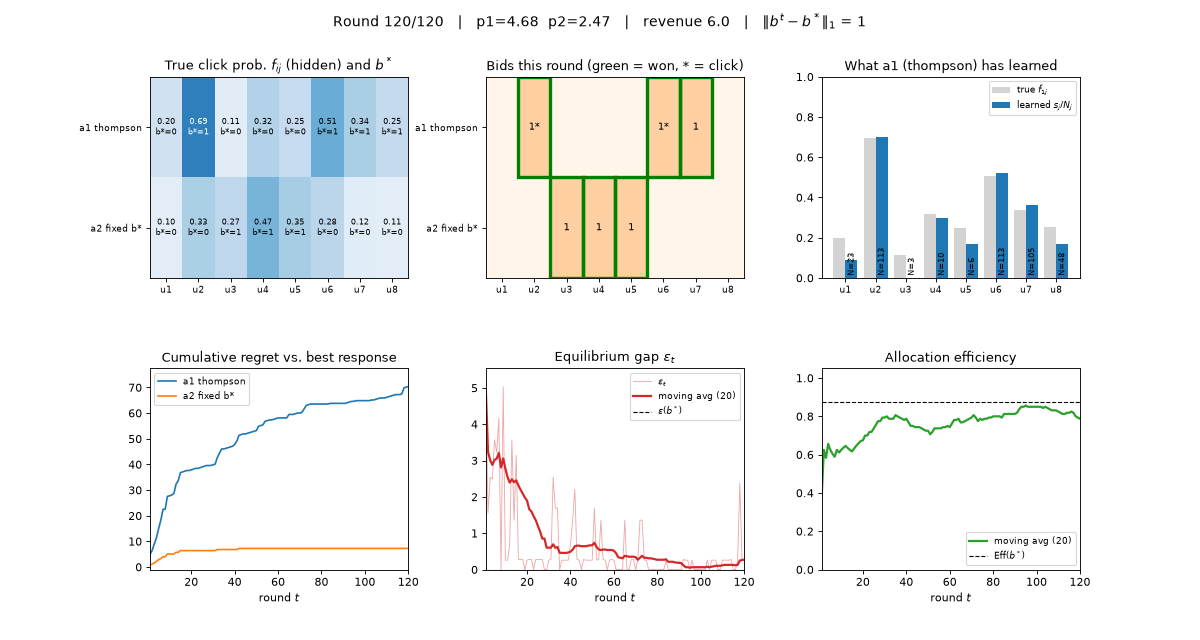
\includegraphics[width=\linewidth]{figures/demo_frame.png}\\[-0.2em]
      {\scriptsize Backup screenshot: Tier 2, Thompson vs.\ fixed $b^*$, $m=2$, $n=8$, $\kappa=0.5$, round 120.}
    \end{column}
  \end{columns}
\end{frame}

\begin{frame}{Takeaways}
  \begin{enumerate}
    \item Learning against a fixed market is cheap: Thompson sampling reaches near-equilibrium
          profit with sublinear regret (slope $\approx 0.3$).
    \item Concurrent learning, not learning itself, is what keeps markets away from $b^*$;
          the effect grows with the number of advertisers.
    \item Budget scarcity hurts efficiency through the equilibrium, not through slower
          learning (H3 rejected as stated).
    \item With a single campaign budget, pacing matters more than the choice of bandit index.
  \end{enumerate}
  \vspace{0.6em}
  \textbf{Future work (brief):} contextual click models shared across users, and win/loss-only
  feedback with random competing bids.
\end{frame}

\begin{frame}{Reproducibility and contributions}
  \small
  \begin{itemize}
    \item \texttt{python run\_evaluation.py sweep \dots} then \texttt{report}: every table and
          figure in the report is regenerated from the sweep outputs; \texttt{python -m pytest}
          runs the tests for all tiers.
    \item Report: \texttt{Doc/report/report.tex} (6 pages) and \texttt{supplementary.tex} (all per-cell tables).
    \item Live demo: \texttt{python run\_demo.py} or \texttt{demo/index.html}.
  \end{itemize}
  \vspace{0.4em}
  \begin{tabular}{@{}ll@{}}
    \toprule
    Vivek Raj & Tier 1: knapsack DP, equilibria, social planner \\
    Anvit Aggarwal & Tier 2: UCB, Thompson, greedy, $\epsilon$-greedy, paced learners \\
    Eshaan Ashish Jaiswal & Tier 3: multi-agent simulator, convergence analysis \\
    Gella Naga Sai Krishna & Evaluation harness, sensitivity study, live demo, report \\
    \bottomrule
  \end{tabular}
\end{frame}

\end{document}
